\section{Analysis}

The process of creation of CERED is mostly an attempt to execute the first two parts of a pipeline we mention in the first chapter \todo{link}. To the best of our knowledge, there is no suitable entity linking tool for Czech. There are tools for Named Entity Recognition that we could theoretically use to our advantage if we decided to focus on named entities only.

Therefore we need to find a way, to get to similar results as the pipeline would get. We do not expect that our CERED generator will be as powerful as the respective dedicated tools would be. We will not try to create a general entity recognition and linking tools - on the contrary, we will exploit any extra information that chosen Wikimedia projects provide.

There are several aspects that we need to think through.
\begin{itemize}
 \item  Dataflow - we already chosen Wikidata and Czech Wikipedia, but we did not discuss how to connect them and what exactly should be the outcome to be able to proceed to locating mentions.
 \item  Entity Matching - suppose we collected a set of entities that could be mentioned in a piece of text and the text. The process of entity matching attemps to mark parts of the text that mention an entity.
 \item  Wikilink mentions - Wikilinks are (mostly) human labeled entity mentions. Utilizing them is the closes we can get to a supervised dataset without actually supervising the dataset.
 \item  Relation Matching - entities are matched, relationships are extracted, can we assume that a sentence with two entities that are related is a mention of this relation? 
\item Relation Inventory - we generated CERED, but the relation inventory is overly diverse. Moreover, the dataset is extremely unbalanced - the number of mentions per relation varies. And no “no relation” relation is obtained.
 \item  Result Evaluation - after each iteration of the development cycle, test are normally run. How to evaluate the consequences of a new feature in the whole CERED?
\end{itemize}



\begin{figure}[h]\centering
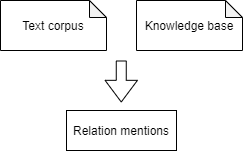
\includegraphics[width=70mm]{./img//Diplomka diagramy-Distant supervision}
\caption{Distant supervision diagram}
\label{obr03:DSD}
\end{figure}

\subsection{Dataflow}

We are starting with two files. One being a Czech Wikipedia dump: it is a collection of articles. Each article has, among other information, its title, id, and text. The other is a Wikidata dump. 

The simplest way of processing those files would be to process them separately and thus obtaining sentences on one side and relationships (a relation type with two items) on the other, see \ref{obr03:DSD} \todo{nene}. This approach comes with a clear disadvantage. We would lose any additional information to the sentences, that could be potentially useful (for example article title might be helpful to determine which items are mentioned in the sentence). To solve this we could precompute something for each article and attach it to each sentence, risking a massive increase in required capacity to work with such data. On a similar note, if we were to follow the diagram exactly, we would probably store item names (labels and aliases) in each relation, worsening the situation even further.

\begin{figure}
\centering
\subfloat[Uninformed approach]{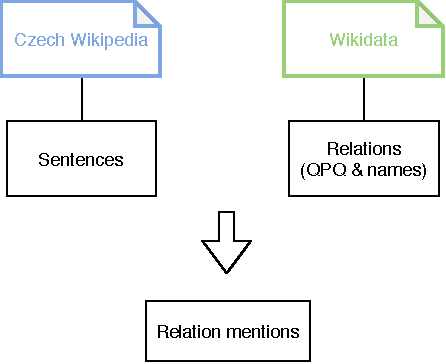
\includegraphics[width=0.4\textwidth]{./img/Diplomka diagramy-uninformed} \label{obr:uninformed}}
\qquad
\subfloat[Informed approach]{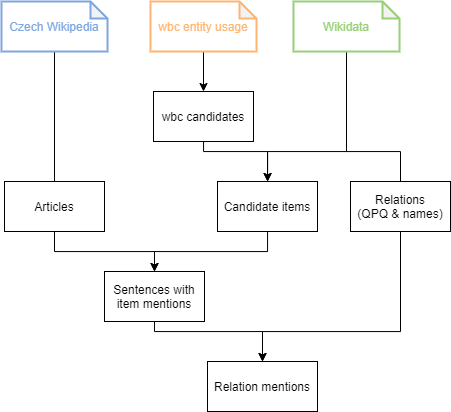
\includegraphics[width=0.6\textwidth]{./img/Diplomka diagramy-informed} \label{obr:informed}}
\label{obr:informedvsuninformed}
\end{figure}



We decided to update the dataflow to address those issues. We will preprocess Wikidata dump to contain only the data we will use. An item will be kept only if it has a Czech name and we will significantly reduce its statements: we will keep the title of its Czech Wikipedia article and create a list of (QID,PID,QID) triples - \defineterm{QPQ}, representing statements that contain information about relations between this and other items. This way, we have all the necessary information - article title to be able to connect an article to an item, names for each item to be able to find mentions of items and finally QPQ triples to connect relations and sentences.

One approach to finding item mentions in text could be called uninformed, see \ref{obr:uninformed}. We could assume that any item can be mentioned in any sentence. This approach seems to have two issues: the computation would likely take quite some time but mainly we expect a huge amount of ambiguous mentions. An example of this ambiguity that we seen as problematic might be children named after their parents. In this case, not only that the entity might get confused, moreover, if we then assign the relation, we might easily confuse a sentence mentioning a spouse relation for a parent relation, which, unfortunately, is extremely challenging to solve. 

On the other side, we can use the extra information that Wikimedia projects provide and opt for a more informed approach. A diagram of this approach is captured in \ref{obr:informed} The topic of most Czech Wikipedia articles is a Wikidata item, therefore this item is nearly certainly mentioned in the article. Some Wikidata statements were based on relevant articles and thus it seems rational to expect items, that are related to the main item of an article, to be mentioned. We decided to look only for a tiny subset of all Wikidata items in each article - \defineterm{candidate items}. As we just discussed, if an article is based on an item, then this item and all items, that are connected to it by a statement, are considered candidate items.

Czech Wikipedia maintains a wbc entity usage table, which contains information about which article uses which item. If we use this table, we are able to obtain a list of items, that should be mentioned in an article, let us call this list a \defineterm{wbc candidates}. A wbc candidate is at the same time a candidate item.

We might consider adding even a second level of relatives (items related to items that are related to the main item) but the branching factor might be relatively high and cause unwanted ambiguity. Consider an instance item like a concrete country, all countries would be second level relatives and thus a candidate item. Since countries tend to be of a certain type (kingdom, republic, state etc.) there might be simply the type or some other more general name amongst their names (\todo{typografie}Q30 United States of America are also known as America or United States) and more countries might share this name.

So far we mostly discussed the advantages of the proposed informed approach, mainly a hope for higher precision specifically higher precision for item mentions. We should elaborate on some disadvantages as well. We are not trying to fully do entity linking. In the end, we will only use item mentions, if the following condition holds: there are two entity mentions in one sentence and a QPQ that connects them exists. It is debatable whether we need an informed approach to increase relation mention precision, the necessity, and improbability that this condition will be fulfilled for false-positive item mentions might in fact be sufficient.

One more way to locate item mentions is trough \defineterm{Wikilinks}. A Wikilink links a page to another page within same-language Wikipedia. First additional information this brings is simply the item mention (if the linked page or article has its main item). We can also consider the textual part of the link to be another name for the linked item. The quality and suitability of this name are to be examined and if we will find these names useful, they can be added to the item names we use.



sice by šlo neparalelně, ale co rychlost?

Mluvit o tom, proč nejdřív najdeme, co v článku hledat, pak to nasekáme na věty, pak matchujeme. Zmínit, kolik je jiných možností, že teoreticky by šlo ještě před rozsekáním na věty dělat entity linking ...

Detailně popsat, co kdy kam poteče + diagram


\subsection{Entity matching}

We have text on one side, gathered candidate items on the other and the goal is to label words that represent those items - entity mentions. There is a wide spectrum of complexity we might aim for, but once again, we are not trying to create a tool for entity recognition and linking. We will describe some of those complexity tears, but before that we should address some basic text manipulation that all of the matching methods will benefit from.



No matter what kind of matching will be done, it seems always beneficial to start with some text preprocessing. Quite a lot of changes need to happen even if some seem like little details. We will separate this preprocessing into a wiki specific part and regular text part. 

\subsubsection{Wikipedia parsing}
Wikipedia is written in Wikitext (Wiki markup, Wikicode). This markup provides all usual functionalities such as determining the layout or fonts and enables commonly-used concepts like lists, links, media file insertion, or tables, and some more wiki specific concepts like infoboxes.

We plan on using some or a combination of existing Wikitext parser since there seems to be a lot of them.\footnote{https://www.mediawiki.org/wiki/Alternative\_parsers} Therefore we believe that the parsing itself will not be troublesome. The more challenging aspect will most likely be deciding, what we consider a valid text for our purpose. From one point of view, a table converted into unstructured text will not be a regular text in terms of sentence structure. From a different point of view, an unstructured text obtained by converting a table still contains information, that human readers will likely decode. Plus, tables or other structured data tend to contain a lot of information. This will likely cause problems because we want to concentrate on sentence-like data, not just for example tuples of data that for example a table of athletes might provide (tuples of persons and countries). This kind of data might significantly damage the quality of CERED.

Eliminating all Wikipedia content, that is too structured or generally, not enough sentence-like, but at the same keeping as much as possible will be addressed while implementing, once we can actually see some statistics about such data.

Wikipedia parsing starts with an article in Wikitext and produces human-readable plain text - \defineterm{clean text}. It should be able to keep track of wikilinks which can be viewed as human-labeled entity mentions.

\subsubsection{Lexical Analysis}
Human-readable text is still not necessarily the best format for our use case. Splitting character sequences into words and sentences is not as easy as we like to think. A tool that addresses such tasks is usually called a tokenizer.
Tokenization is a process that aims to split text (sequence of characters) into separate tokens. Naive tokenizer might just simply split on non-alphanumeric characters. But if the tokenizer is supposed to actually perform well and recognize sentences, a way more sophisticated tool is needed. For this reason, we will outsource handling text to a Czech tokenizer called MorphoDiTa, reasons for choosing this specific tokenizer will be discussed in \todo{link}. Using MorphoDiTa tokenization, we can convert clean text into sentences made up of tokens and we even obtain the lemma and lexeme of each token.

\subsubsub{Lexical Analysis on Names}. Tokenizers (and lemmatizers) are usually trained to perform well on sentences and might be inaccurate on noun phrases when they stand alone, as entity names do. If we were determined to tokenize them a simple trick like constructing a sentence with the name in it and tokenizing this sentence can partially solve this problem. Such sentence that would be grammatically correct and not semantically terrible could be something like “This is /name/”, but realistically, this sentence was quite likely not at all common in the training process of MorphoDiTa. Some foreign words can be erroneous as well and keeping their original form might be the only easy way around it.

\subsubsection{Matching methods}
Entity matching can be done with various degrees of sophistication. We provide a short overview of those degrees, focusing mainly on those that are to be implemented. For simplicity, we will assume that we are only looking for mentions in one sentence at a time unless written otherwise. We also include an example of such matchings to demonstrate how unsuccessful we are likely to be.

\begin{figure}

Lord Voldemort (Tom Rojvol Raddle, Voldemort, Pán zla)

\caption{First paragraph from Czech Wikipedia page about Lord Voldemort Q176132, also known as Tom Rojvol Raddle, Voldemort, Pán zla (Dark Lord) }


\end{figure}
\todo{značka pro překlad v caption} 

\subsubsub{String equality}. Definitely the easiest method of entity matching. This method is based on a simple substring check which is later extended with additional functionality. In more detail, for each entity, we have multiple name strings and for each of those names, we check whether the name is a substring of the sentence.

We still need to work with letter cases. Named entities should have a fixed letter cases and no additional processing is needed in most cases. In other cases, an established name for a named entity might be written with the lowercased first letter (Weasley family (Q716534) has Czech names 'Weasleyovi' /the Weasleys/ but also rodina Weasleyových /Weasley family/, but there are examples where those different names are completely different (\todo{český} Elizabeth II and Queen of England would be translated to Alžběta II. and královna Anglie). If we consider entities, that are commonly written with lower case (\todo{příklady jako škola, tužka}), the sentence now needs to be preprocessed so that for example the first letter is not capital. Moreover, there is no guarantee that common names will be lowercased in Wikidata. To conclude, nearly nothing can be assumed about the case of letters, and therefore one of the following solutions needs to be implemented: everything can be converted to one chosen letter case or some more sophisticated attempts at predicting, which words can have more version in terms of letter cases.

Spaces come with issues as well especially if combined with previous tokenization. We will list some troublesome examples and accept the fact that not everything can be done perfectly. J. K. Rowling has J.K.Rownling as one of Wikidata names, confirming that both versions might appear in written text, but not all entities with similar name type have all space-variants listed in names. We assume that spacing around the ‘-’ \todo{-} character might vary.

It is also not clear if word order in names is fixed for at least for nearly all entity mentions. Even the simple reversion in name, that is sometimes used, will affect the performance of this method (J. K. Rowling and Rowling, J. K.).  Even cases where the name is divided by for example apposition into two separate parts might exist.

The greatest weakness of this method is its inability to recognize entities if their name is inclined. To empathize how many words are not in the same form as their lemma in Czech text, we colored them in the sample text. \todo{vybarvit a dát link} We elaborated on Czech language in \todo{link} CHAPTER XX, but just for simplicity - in English the verb to be has many different forms (am, are, were, was, would and so on), all nouns and verbs in Czech behave like this, quite often with many more forms.

\subsubsub{String similarity (approximate string matching)} String similarity is still based on simple string manipulation, no vocabulary or other language knowledge is necessary. The goal is to find entity mention, even if its name is a little altered in the sentence. This alternation can include all of the issues listed for the previous method - cases of letters, spacing, word order, and word forms, but even better, it might help in cases, that we did not anticipate.

There are many metrics describing string similarity. Some could cope better with word order issues, some with word forms, some with spacing. We will not test all of them for our usecase, but still find it useful to mention them since in other than the Czech language, some might work well.

\defineterm{Edit distance}. First category of string similarity metric is based on edit distance:

Levenshtein distance is the minimum number of edits (additions, deletions, and substitutions of a character) to get from one string to the other. As a metric the ratio of Levenshtein distance and of the sum of the lengths of the strings can be used. This metric, unsurprisingly, deals well with mentions that are close to the names when it comes to the amount of edits needed, so mentions differentiating in a word form, different spacing, or letter casing will could be considered a match.

Damerau–Levenshtein distance is very similar to the previous, but a transposition of two adjacent characters is considered an edit. We might argue that some Czech words tend to transpose the last characters in different word forms and thus this metric could work better for those forms, but there might be a higher risk of false positives.

One more thing to mention about edit distances is that they count the distance of two string, in our case of a name and of a substring of a sentence, because we do not expect an entire sentence to be entity mention. Therefore we need to decide on a logic for choosing substrings of a sentence to count the distance on, without diving too deep into this, the time complexity (even though both the sentence and the name length is relatively small) can be high if we consider the amount of data we need to process. (Let $s, n$ be lengths of a sentence and a name, there are $s^2/2$ substrings and each edit distance can be computed in $sn$, leading to $s^3n$). \todo{vynechat}

\defineterm{Token based}. Another category is based on tokens. For those metrics, we can either use the tokenized sentences (by an actual tokenizer) and try to tokenize names, so that the format matches, or we can use naive tokenization like removing non-alphanumeric character and splitting on spaces.

The tokenization converts both the sentence string and the name string into a set of tokens ($S, N$ respectively), so metrics that work with sets can be utilized: Intersection over union is computed as $|S \cap N| / |S \cup N|$. Any other set similarity measure can be used. 

Token based metrics - due to their set nature - ignore the order of tokens and therefore could solve issues with mentions in which the word order is not the same as in the name. On the other side, an increase in false positives is to be expected and some additional postprocessing is needed to determine which token in the sentence should be considered a mention if the token was used in the sentence multiple times. We also feel obligated to mention that once again, we are not trying to find the similarity of a sentence and a name, but of a substring of a sentence and a name. This leads to the idea of removing all tokens, that are in a sentence and would worsen the metric and in result modifying the formula for intersection over union to  $|S \cap N| / |N|$.


\defineterm{Sequence based}. Just to be a bit more comprehensive we include another type of metrics - sequence based, even though we doubt that it is the best approach for entity matching. They ignore words as wholes and we do not see any advantage of those metrics for our use case. 

Ratcliff-Obershelp similarity finds the longest common substring that is longer than some limit and recursively does so for the non-common parts of strings. The result is based on the ratio of (double the) length of common parts and overall length. 

Bigram (or n-gram) intersection over union which converts both strings into a set of n-grams (n adjecant characters) and performs intersection over union. This time reducing a sentence into a substring is not that straight forward and would require additional attention.


\subsubsub{Morphological analysis}
Moving on from methods that are mostly unaware of the language they work with, we will finally use the morphological analysis we mention earlier.

With lemmas of both the sentence and the name, we can use any metric from the previous subsection on string similarity (joining the lemmas if a single two strings are needed).

If we decide to keep the names in their original form (tokenization on them can be error prone, as we already explained), we can try to use the correct form of the tokens in the sentence. For each lemma, we get a set of all its possible forms - a lexeme, now we can modify the previous metrics to work with lexemes instead of tokens. 

\subsubsub{Advanced concepts}

A proper entity matching (either in named entity recognition or entity linking) might be expected to recognize entity mention even if the entity is not mentioned explicitly by its name. Pronounces should be assigned an entity they represent (if they do) and other nouns as well. In languages like Czech where the subject of a sentence is often omitted the entity mention is even less obvious but still present. Since the topic of this thesis is not entity matching, we will not debate techniques to achieve this level of matching neither will we implement them.

\todo{mezera}
\vspace{2mm}
We ended up using a rather simple metric after looking at the results, but we still find it useful to keep this summarization of different string metrics as part of this thesis. A detailed description of the matching method CERED was generated with is written in XX \todo{YY}.

\todo{
Napsat, že v aj dělají často jen exact modulo zkratky a malé přípony, což tady nejde.

Ukázat nápady se sebráním linků z wikipedie a zavrhnout to

připomenout, jak moc se dá čeština skloňovat
říct, že nemá nejspíš smysl snažit se najít jen validní tvary, protože stejně v textu nejspíš nebudou nevalidní

asi mluvit o word order? a možná i implementovat

Říct, že jako kontrolní dataset budou přímo z linků}

\subsection{Wikilink Mentions}

As we already mentioned, from our point of view Wikilinks are entity mentions created by Wikipedia editors. The text part of the link can in theory be anything providing us with some more advanced examples of entity linking, that our matching methods cannot perform.

V pátém díle McGonagallová říká, že předmět vyučuje již 39 let

We want to enable the users of CERED to distinguish relation mentions that were created based on two Wikilinks from all others. Since this data is not fully supervised and the word supervised is used often \todo{přetížený} (semi-supervised, distant-supervised, etc.) we decided to call it \defineterm{silver}, because they are not of the optimal quality that is usually labeled gold, but they are the best we can get.


\subsection{Relation Matching}
If a sentence contains two entity mentions that are related, chances are that the sentence in fact does express their relationship and thus is a relation mention. This concept is called \defineterm{distatnt supervision assumption} and can be also formulated in the following was: If two entities participate in a relation, all sentences that  mention these two entities express that relation. The reason why this assumption is used, even though it is clearly not correct, is how easy it is to use. To tell how often this assumption is violated is labor-intensive, luckily research has been done on this topic. In the \cite{nytdistant} \todo{link} the distant supervision assumption is compared to an \defineterm{express-at-least-once assumption} which states that if two entities participate in a relation, at least one sentence that mentions these two entities might express that relation. 

They sampled 600 relation mentions from two corpora, both created by distant supervision on Freebase (knowledge base commonly used before Wikidata took over) and two text corpora - Wikipedia articles and the New York Times corpus. Those 600 samples represented three different relation types (nationality, place of birth, and contains) and were sampled so that there were 100 samples of each type in each corpus. We include their results in table XX \todo{table} They concluded that Wikipedia is a very specific type of text corpora, because articles are centered around entities. We believe that the reasoning can be extended with the fact, that freebase contained information from Wikipedia infoboxes, and those infoboxes were created based on the textual information. 

For the authors the results signalized that a more sophisticated tool is needed instead of relying on the distant supervision assumption. We acknowledge that such a tool is needed but at the same time we believe that in our case, where we create CERED based on Wikipedia and Wikidata, the precision they estimated is sufficient. We also assume that Wikidata project is more suitable for this task than was Freebase.

We want to mention that we build CERED to easily fit into the modern deep learning models and to be as simple as possible. Therefore the main piece of text we use is a sentence, it might seem intuitive, but it has one downfall. If the relationship extractor was to be used on a real text not to determine where some relations are mentioned but to provide a summary of relations expressed by the text as a whole, some information will be lost. \todo{najít článek nebo někam přesunout?}

\subsection{Relation Inventory}
In chapter XX some examples of Relationship classification datasets were introduced. The creators of those datasets claim that in the creation process they first decided on the relation inventory (relation types).  Creating the relation inventory seems to be the straight forward and rational approach and we wanted to create such inventory before actually implementing the CEDER generator. We stumbled on the following issues.

\subsubsub{Issue 1}Wikidata relation inventory (properties in Wikidata terminology) is an order of magnitude larger compared to the traditional relationship extraction datasets and handpicking our inventory is overwhelming. We even considered reducing the size of this inventory by creating our own relationships that would combine Wikidata properties (parent would be the combination of mother and father relations). 

By restricting the Wikidata inventory to just some properties we reduce the size of CERED and if we choose the inventory without considering the number of mentions per relationship, the best-represented relations could be omitted.

\subsubsub{Issue 2}Knowledge basis, in general, do not contain negative relations (such relations that could be easily mapped to the “no relation” or “other relation”\todo{typografie}), but for relationship extraction negative mentions are essential. If we generate mentions using all properties we can later decide which relationships will be in the inventory and the rest of them relabel to “other relation” \todo{typografie}. If we were to assign all tuples of entity mentions that share a sentence and are not related as “no\_relationship”, we could increase the noise in CERED because not all relationships are in Wikidata and therefore part of the no\_relationship mentions could in fact be a positive mention. The commonly used ratio of negative and positive mentions is \todo{kolik?}.

While curating the inventory, we should keep in mind, that we are not just choosing the relations but also their representations and we need to attempt to fulfill the three following requirements to the best of our abilities:
\begin{itemize}
\item Each relation needs to be represented enough.
\item The more balanced relation representation sizes the better.
\item There should be enough negative mentions and their negativity should be assured. \todo{reformulovat}

\end{itemize}

\subsection{Result Evaluation}
The by far most challenging aspect of working Czech Wikipedia and Wikidata is their size and diversity. To the best of our knowledge there is no strictly followed guideline when it comes to editing either the articles or item information. Just converting Wikipedia dump to clean text will be challenging due to user defined templates and other constructs we might be unaware of. On the other side names in Wikidata can be too general (like someone first name) and create false entity mentions. 

We prepared several metrics and methods to measure the quality of the implemented generator and we will list them in the table \ref{tab:qualityEval}. Unfortunately going through the article and seeing what did and did not get recognized as a mention is still the most powerful method, therefore we decided to develop a simple app that can prettify the output of the generator and makes the process of looking at the results less painful. \todo{příliš neformální?} 

\begin{figure}

\begin{tabular}{p{0.05\linewidth}p{0.8\linewidth}}

FA & The overall count of found mentions - to some extent the greater the better - at least in the beginning with naive matching methods. With more sophisticated matching, this number should increase. On the other side, this measure will decrease with more precise Wikitext manipulation. \\ 
FA & If the distribution of the amount of found mentions (both the entity mentions before relation matching and the relation mentions) over some domain is peculiar (contains abnormalities such unexpected peeks) the quality of not only those mentions might be lower. The domain can be anything from the following or even multiple of them at the same time:
sentence, article, relation, entity, sentence number (the order of the sentence in an article), entity pair. \\ 
NA & Checking the anomalies detected by the previous methods.  \\ 
NA & Checking an article and realizing what did and didn't get matched. \\ 
FA & Some articles could be labeled by hand and test could be created.\\

\end{tabular} 

\caption{Quality evaluation methods and the potential for automatization (Fully Automatic, Not-Automatic)}
\label{tab:qualityEval}
\end{figure}


\subsubsection{Viewer}

The purpose of this viewer is to present the results in a more graphical way to fasten and pleasant the process of checking them, which will be done often and will take a significant amount of time.

We want the viewer to be able to show the statistics about the generated data, that were collected during the generation, the configuration that was used to generate the dataset, and mainly to show an article with the found mentions (entity and relation). 

Streamlit made implementing such viewer quite easy and we used spaCy’s \todo{footnote} visualizations. \todo{přestěhovat někam dopryč tento odstavec}

\todo{screen viewertu k implementaci}





\begin{figure}[p]\centering
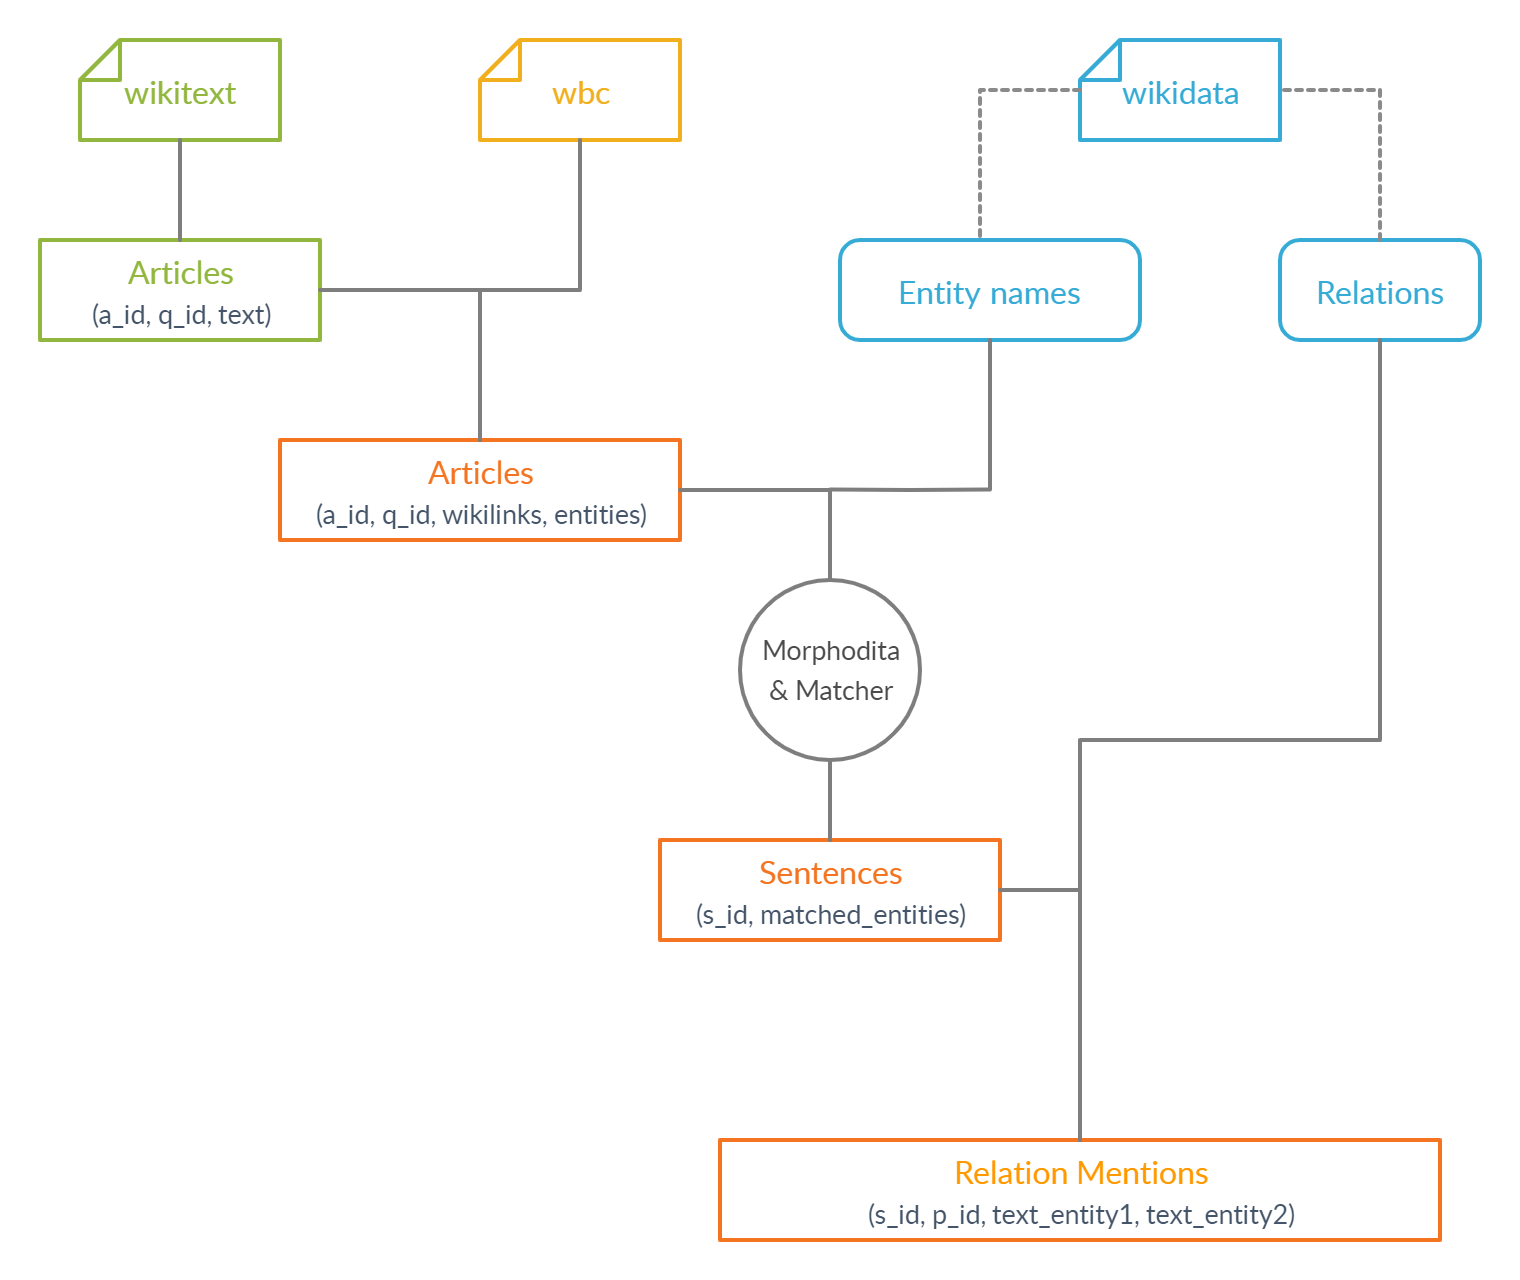
\includegraphics[width=140mm, height=117mm]{./img/Corpus_diagram}
\caption{Zjednodušený diagram výroby korpusu}
\label{obr03:Nhust}
\end{figure}

\todo{do sekce o češtině přidat velká malá pismenka}

https://www.aclweb.org/anthology/P19-1074.pdf
